\subsubsection{Parasitäre Paramter}\label{subsec:parasitparam}
In diesem Unterkapitel werden grundsätzlich die Einflüsse und Eigenschaften von Parasitären Paramentern in Realen Bauteilen, besonders Spule und Kondensator, erklärt.

Ideale Bauteile beschreiben eine Funktion. Da reale Bauteile aus Materialien mit physikalischen Eigenschaften bestehen, treten bei der Umsetzung dieser Funktion Nebeneffekte auf. Sie entstehen, weil die einzelnen Bauteile im Betrieb elektrische Felder oder Magnetfelder erzeugen. Oder einfach durch die Leitfähigkeit eines Materials. Diese physikalisch bedingten Effekte werden als parasitär bezeichnet. Sie treten als Widerstand, Induktivität oder Kapazivität auf. Da sie gut klassifiziert werden können, werden sie als Parameter bezeichnet. 
Um eine Schaltung präzise zu simulieren ist es unerlässlich, die elektrischen Bauelemente mit den passenden parasitären Parametern zu ergänzen. In den Abbildungen \ref{fig:stray_L} und \ref{fig:stray_C} werden die parasitären Parameter von Spule und Kondensator gezeigt. Man stellt sie als zusätzliche Bauteile dar. \textcolor{red}{\textbf{TODO:Quelle ganzes kapitel}}


\begin{figure}[H]
	\begin{minipage}[h]{0.45\linewidth}
		\centering
		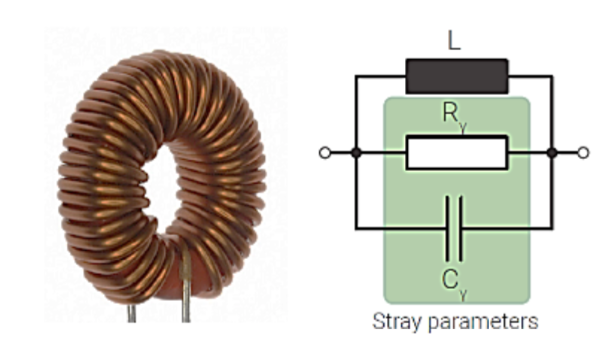
\includegraphics[width = 5cm]{stray_L.png}
		\caption{Parasiäre Elemente einer Induktivität \cite{aufgabenstellung}}
		\label{fig:stray_L}
	\end{minipage}	
	\begin{minipage}[h]{0.45\linewidth}
		\centering
		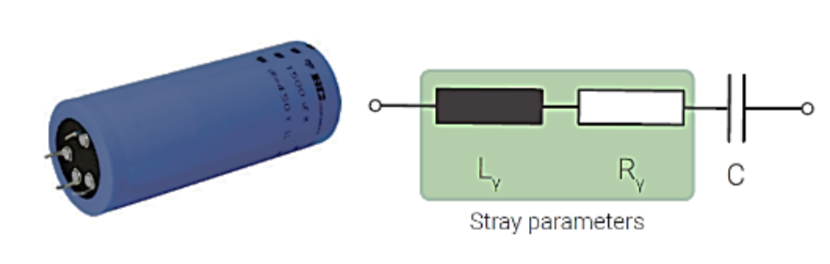
\includegraphics[width = 7cm]{stray_C.png}
		\caption{Parasiäre Elemente einer Kapazität \cite{aufgabenstellung}}
		\label{fig:stray_C}
	\end{minipage}
\end{figure}

\bigskip
